\PassOptionsToPackage{unicode=true}{hyperref} % options for packages loaded elsewhere
\PassOptionsToPackage{hyphens}{url}
%
\documentclass[ignorenonframetext,]{beamer}
\usepackage{pgfpages}
\setbeamertemplate{caption}[numbered]
\setbeamertemplate{caption label separator}{: }
\setbeamercolor{caption name}{fg=normal text.fg}
\beamertemplatenavigationsymbolsempty
% Prevent slide breaks in the middle of a paragraph:
\widowpenalties 1 10000
\raggedbottom
\setbeamertemplate{part page}{
\centering
\begin{beamercolorbox}[sep=16pt,center]{part title}
  \usebeamerfont{part title}\insertpart\par
\end{beamercolorbox}
}
\setbeamertemplate{section page}{
\centering
\begin{beamercolorbox}[sep=12pt,center]{part title}
  \usebeamerfont{section title}\insertsection\par
\end{beamercolorbox}
}
\setbeamertemplate{subsection page}{
\centering
\begin{beamercolorbox}[sep=8pt,center]{part title}
  \usebeamerfont{subsection title}\insertsubsection\par
\end{beamercolorbox}
}
\AtBeginPart{
  \frame{\partpage}
}
\AtBeginSection{
  \ifbibliography
  \else
    \frame{\sectionpage}
  \fi
}
\AtBeginSubsection{
  \frame{\subsectionpage}
}
\usepackage{lmodern}
\usepackage{amssymb,amsmath}
\usepackage{ifxetex,ifluatex}
\usepackage{fixltx2e} % provides \textsubscript
\ifnum 0\ifxetex 1\fi\ifluatex 1\fi=0 % if pdftex
  \usepackage[T1]{fontenc}
  \usepackage[utf8]{inputenc}
  \usepackage{textcomp} % provides euro and other symbols
\else % if luatex or xelatex
  \usepackage{unicode-math}
  \defaultfontfeatures{Ligatures=TeX,Scale=MatchLowercase}
\fi
% use upquote if available, for straight quotes in verbatim environments
\IfFileExists{upquote.sty}{\usepackage{upquote}}{}
% use microtype if available
\IfFileExists{microtype.sty}{%
\usepackage[]{microtype}
\UseMicrotypeSet[protrusion]{basicmath} % disable protrusion for tt fonts
}{}
\IfFileExists{parskip.sty}{%
\usepackage{parskip}
}{% else
\setlength{\parindent}{0pt}
\setlength{\parskip}{6pt plus 2pt minus 1pt}
}
\usepackage{hyperref}
\hypersetup{
            pdfauthor={Peter Gao},
            pdfborder={0 0 0},
            breaklinks=true}
\urlstyle{same}  % don't use monospace font for urls
\newif\ifbibliography
\usepackage{color}
\usepackage{fancyvrb}
\newcommand{\VerbBar}{|}
\newcommand{\VERB}{\Verb[commandchars=\\\{\}]}
\DefineVerbatimEnvironment{Highlighting}{Verbatim}{commandchars=\\\{\}}
% Add ',fontsize=\small' for more characters per line
\usepackage{framed}
\definecolor{shadecolor}{RGB}{248,248,248}
\newenvironment{Shaded}{\begin{snugshade}}{\end{snugshade}}
\newcommand{\AlertTok}[1]{\textcolor[rgb]{0.94,0.16,0.16}{#1}}
\newcommand{\AnnotationTok}[1]{\textcolor[rgb]{0.56,0.35,0.01}{\textbf{\textit{#1}}}}
\newcommand{\AttributeTok}[1]{\textcolor[rgb]{0.77,0.63,0.00}{#1}}
\newcommand{\BaseNTok}[1]{\textcolor[rgb]{0.00,0.00,0.81}{#1}}
\newcommand{\BuiltInTok}[1]{#1}
\newcommand{\CharTok}[1]{\textcolor[rgb]{0.31,0.60,0.02}{#1}}
\newcommand{\CommentTok}[1]{\textcolor[rgb]{0.56,0.35,0.01}{\textit{#1}}}
\newcommand{\CommentVarTok}[1]{\textcolor[rgb]{0.56,0.35,0.01}{\textbf{\textit{#1}}}}
\newcommand{\ConstantTok}[1]{\textcolor[rgb]{0.00,0.00,0.00}{#1}}
\newcommand{\ControlFlowTok}[1]{\textcolor[rgb]{0.13,0.29,0.53}{\textbf{#1}}}
\newcommand{\DataTypeTok}[1]{\textcolor[rgb]{0.13,0.29,0.53}{#1}}
\newcommand{\DecValTok}[1]{\textcolor[rgb]{0.00,0.00,0.81}{#1}}
\newcommand{\DocumentationTok}[1]{\textcolor[rgb]{0.56,0.35,0.01}{\textbf{\textit{#1}}}}
\newcommand{\ErrorTok}[1]{\textcolor[rgb]{0.64,0.00,0.00}{\textbf{#1}}}
\newcommand{\ExtensionTok}[1]{#1}
\newcommand{\FloatTok}[1]{\textcolor[rgb]{0.00,0.00,0.81}{#1}}
\newcommand{\FunctionTok}[1]{\textcolor[rgb]{0.00,0.00,0.00}{#1}}
\newcommand{\ImportTok}[1]{#1}
\newcommand{\InformationTok}[1]{\textcolor[rgb]{0.56,0.35,0.01}{\textbf{\textit{#1}}}}
\newcommand{\KeywordTok}[1]{\textcolor[rgb]{0.13,0.29,0.53}{\textbf{#1}}}
\newcommand{\NormalTok}[1]{#1}
\newcommand{\OperatorTok}[1]{\textcolor[rgb]{0.81,0.36,0.00}{\textbf{#1}}}
\newcommand{\OtherTok}[1]{\textcolor[rgb]{0.56,0.35,0.01}{#1}}
\newcommand{\PreprocessorTok}[1]{\textcolor[rgb]{0.56,0.35,0.01}{\textit{#1}}}
\newcommand{\RegionMarkerTok}[1]{#1}
\newcommand{\SpecialCharTok}[1]{\textcolor[rgb]{0.00,0.00,0.00}{#1}}
\newcommand{\SpecialStringTok}[1]{\textcolor[rgb]{0.31,0.60,0.02}{#1}}
\newcommand{\StringTok}[1]{\textcolor[rgb]{0.31,0.60,0.02}{#1}}
\newcommand{\VariableTok}[1]{\textcolor[rgb]{0.00,0.00,0.00}{#1}}
\newcommand{\VerbatimStringTok}[1]{\textcolor[rgb]{0.31,0.60,0.02}{#1}}
\newcommand{\WarningTok}[1]{\textcolor[rgb]{0.56,0.35,0.01}{\textbf{\textit{#1}}}}
\usepackage{graphicx,grffile}
\makeatletter
\def\maxwidth{\ifdim\Gin@nat@width>\linewidth\linewidth\else\Gin@nat@width\fi}
\def\maxheight{\ifdim\Gin@nat@height>\textheight\textheight\else\Gin@nat@height\fi}
\makeatother
% Scale images if necessary, so that they will not overflow the page
% margins by default, and it is still possible to overwrite the defaults
% using explicit options in \includegraphics[width, height, ...]{}
\setkeys{Gin}{width=\maxwidth,height=\maxheight,keepaspectratio}
\setlength{\emergencystretch}{3em}  % prevent overfull lines
\providecommand{\tightlist}{%
  \setlength{\itemsep}{0pt}\setlength{\parskip}{0pt}}
\setcounter{secnumdepth}{0}

% set default figure placement to htbp
\makeatletter
\def\fps@figure{htbp}
\makeatother


\setbeamercolor{red1}{fg = white, bg=pink}
\definecolor{bluebell}{rgb}{0.64, 0.64, 0.82}
\definecolor{coralred}{rgb}{1.0, 0.25, 0.25}
\definecolor{apricot}{rgb}{0.98, 0.81, 0.69}
\setbeamercolor{itemize item}{fg=black}


%%%% HEADLINE %%%%
\makeatletter
\setbeamertemplate{navigation symbols}{}
\setbeamercolor{head}{fg=black}
\setbeamertemplate{headline}
{
	\leavevmode%
	\hbox{%
		\begin{beamercolorbox}[wd=.5\paperwidth,ht=3ex,dp=2ex, left]{head}%
			\usebeamerfont{foot}
			\hspace{1ex}Lecture 03 \insertsection
		\end{beamercolorbox}%
		
		\begin{beamercolorbox}[wd=.5\paperwidth,ht=3ex,dp=2ex,right]{head}%
			\usebeamerfont{foot}
			Summarizing Data\hspace*{2ex} 
	\end{beamercolorbox}}%
	\vskip1pt%
}
\makeatother

%%%% FOOTLINE %%%%
\makeatletter
\setbeamertemplate{navigation symbols}{}
\setbeamercolor{foot}{fg=black}
\setbeamertemplate{footline}
{
	\leavevmode%
	\hbox{%
		\begin{beamercolorbox}[wd=.5\paperwidth,ht=3ex,dp=1ex, left]{foot}%
			\usebeamerfont{foot}
			\hspace{1ex}Q SCI 381 \insertsection
		\end{beamercolorbox}%

		\begin{beamercolorbox}[wd=.5\paperwidth,ht=3ex,dp=1ex,right]{foot}%
			\usebeamerfont{foot}
			\insertframenumber{}\hspace*{2ex} 
	\end{beamercolorbox}}%
	\vskip1pt%
}
\makeatother

\setbeamertemplate{caption}{\footnotesize{\raggedright\insertcaption\par}}

\usepackage{fontspec}
\newfontfamily{\gar}{Marion}
\setsansfont{Helvetica Neue}

\usepackage{etoolbox}
\usepackage{enumitem}
\BeforeBeginEnvironment{frame}{%
  \setbeamercolor{background canvas}{bg=white}
  \setbeamercolor{head}{fg=black}
  \setbeamercolor{foot}{fg=black}
}
\makeatletter
\define@key{beamerframe}{standout}[true]{%
  \setbeamercolor{background canvas}{bg=bluebell}
  \setbeamercolor{head}{fg=white}
  \setbeamercolor{foot}{fg=white}
}
\makeatother

\author{Peter Gao}
\date{6/17/2020}

\begin{document}

\begin{frame}{}
\protect\hypertarget{section}{}

\vspace{4em}
\Large{\textbf{Introduction to Probability and Statistics}}

\vspace{3em}
\footnotesize

\textit{26 June 2020}

\end{frame}

\begin{frame}[standout]{}
\protect\hypertarget{section-1}{}

\color{apricot}\textit{\gar\Huge recap}

\normalsize\color{white}\vspace{4ex}\textbf{ Last lecture, we discussed:}

\vspace{2ex}
\begin{itemize}
\color{white}
\setlength{\itemsep}{2ex}
\item Types of studies
\item Types of sampling
\item Principles of experimental design
\end{itemize}

\end{frame}

\begin{frame}[standout]{}
\protect\hypertarget{section-2}{}

\color{apricot}\textit{\gar\Huge recap}

\scriptsize \color{white}
\vspace{4ex}

Suppose we want to estimate household size, where a ``household'' is
defined as people living together in the same dwelling, and sharing
living accommodations.

\vspace{2ex}

If we select students at random at an elementary school and ask them
what their family size is,
\textbf{will this be a good measure of household size}? Or will our
average be biased? If so, will it overestimate or underestimate the true
value?

\vspace{2ex}

\hfill(\textit{OpenIntro Statistics}, exercise 1.26)

\end{frame}

\begin{frame}[standout]{}
\protect\hypertarget{section-3}{}

\begin{center}
        
    \vspace{2.3em}
    \color{white}\textit{\Huge\gar Summarizing data}
\end{center}

\end{frame}

\begin{frame}[fragile]{}
\protect\hypertarget{section-4}{}

\scriptsize

\begin{Shaded}
\begin{Highlighting}[]
\CommentTok{# load food consumption dataset }
\NormalTok{food_consumption <-}
\StringTok{  }\NormalTok{readr}\OperatorTok{::}\KeywordTok{read_csv}\NormalTok{(}
    \KeywordTok{paste0}\NormalTok{(}\StringTok{'https://raw.githubusercontent.com/'}\NormalTok{,}
           \StringTok{'rfordatascience/tidytuesday/master/'}\NormalTok{,}
           \StringTok{'data/2020/2020-02-18/food_consumption.csv'}\NormalTok{)}
\NormalTok{    )}
\end{Highlighting}
\end{Shaded}

\end{frame}

\begin{frame}[fragile]{}
\protect\hypertarget{section-5}{}

\textbf{\large Food Consumption data}

Data from the the United Nations on the \textbf{annual per-capita}
consumption of eleven categories of food for 130 countries.

\vspace{1ex}\scriptsize

\begin{Shaded}
\begin{Highlighting}[]
\KeywordTok{unique}\NormalTok{(food_consumption}\OperatorTok{$}\NormalTok{country)}
\end{Highlighting}
\end{Shaded}

\begin{verbatim}
##   [1] "Argentina"              "Australia"             
##   [3] "Albania"                "Iceland"               
##   [5] "New Zealand"            "USA"                   
##   [7] "Uruguay"                "Luxembourg"            
##   [9] "Brazil"                 "Kazakhstan"            
##  [11] "Sweden"                 "Bermuda"               
##  [13] "Denmark"                "Finland"               
##  [15] "Ireland"                "Greece"                
##  [17] "France"                 "Canada"                
##  [19] "Norway"                 "Hong Kong SAR. China"  
##  [21] "French Polynesia"       "Israel"                
##  [23] "Switzerland"            "Netherlands"           
##  [25] "Kuwait"                 "United Kingdom"        
##  [27] "Austria"                "Oman"                  
##  [29] "Italy"                  "Bahamas"               
##  [31] "Portugal"               "Malta"                 
##  [33] "Armenia"                "Slovenia"              
##  [35] "Chile"                  "Venezuela"             
##  [37] "Belgium"                "Germany"               
##  [39] "Russia"                 "Croatia"               
##  [41] "Belarus"                "Spain"                 
##  [43] "Paraguay"               "New Caledonia"         
##  [45] "South Africa"           "Barbados"              
##  [47] "Lithuania"              "Turkey"                
##  [49] "Estonia"                "Mexico"                
##  [51] "Costa Rica"             "Bolivia"               
##  [53] "Ecuador"                "Panama"                
##  [55] "Czech Republic"         "Romania"               
##  [57] "Colombia"               "Maldives"              
##  [59] "Cyprus"                 "Serbia"                
##  [61] "United Arab Emirates"   "Algeria"               
##  [63] "Ukraine"                "Pakistan"              
##  [65] "Swaziland"              "Latvia"                
##  [67] "Bosnia and Herzegovina" "Fiji"                  
##  [69] "South Korea"            "Poland"                
##  [71] "Saudi Arabia"           "Botswana"              
##  [73] "Macedonia"              "Hungary"               
##  [75] "Trinidad and Tobago"    "Tunisia"               
##  [77] "Egypt"                  "Mauritius"             
##  [79] "Bulgaria"               "Morocco"               
##  [81] "Slovakia"               "Niger"                 
##  [83] "Kenya"                  "Jordan"                
##  [85] "Japan"                  "Georgia"               
##  [87] "Grenada"                "El Salvador"           
##  [89] "Cuba"                   "China"                 
##  [91] "Honduras"               "Taiwan. ROC"           
##  [93] "Angola"                 "Jamaica"               
##  [95] "Namibia"                "Belize"                
##  [97] "Malaysia"               "Zimbabwe"              
##  [99] "Guatemala"              "Uganda"                
## [101] "Nepal"                  "Iran"                  
## [103] "Tanzania"               "Senegal"               
## [105] "Peru"                   "Nicaragua"             
## [107] "Vietnam"                "Ethiopia"              
## [109] "Myanmar"                "Congo"                 
## [111] "Zambia"                 "Cameroon"              
## [113] "Madagascar"             "Malawi"                
## [115] "Guinea"                 "Nigeria"               
## [117] "Rwanda"                 "Philippines"           
## [119] "Ghana"                  "Togo"                  
## [121] "Gambia"                 "India"                 
## [123] "Thailand"               "Mozambique"            
## [125] "Cambodia"               "Sierra Leone"          
## [127] "Sri Lanka"              "Indonesia"             
## [129] "Liberia"                "Bangladesh"
\end{verbatim}

\end{frame}

\begin{frame}[fragile]{}
\protect\hypertarget{section-6}{}

\textbf{\large Food Consumption data}

\vspace{1ex}\scriptsize

\begin{Shaded}
\begin{Highlighting}[]
\NormalTok{food_consumption }\OperatorTok
\StringTok{  }\KeywordTok{filter}\NormalTok{(country }\OperatorTok{==}\StringTok{ "USA"}\NormalTok{)}
\end{Highlighting}
\end{Shaded}

\begin{verbatim}
## # A tibble: 11 x 4
##    country food_category            consumption co2_emmission
##    <chr>   <chr>                          <dbl>         <dbl>
##  1 USA     Pork                           27.6          97.8 
##  2 USA     Poultry                        50.0          53.7 
##  3 USA     Beef                           36.2        1118.  
##  4 USA     Lamb & Goat                     0.43         15.1 
##  5 USA     Fish                           12.4          19.7 
##  6 USA     Eggs                           14.6          13.4 
##  7 USA     Milk - inc. cheese            255.          363.  
##  8 USA     Wheat and Wheat Products       80.4          15.3 
##  9 USA     Rice                            6.88          8.8 
## 10 USA     Soybeans                        0.04          0.02
## 11 USA     Nuts inc. Peanut Butter         7.86         13.9
\end{verbatim}

\end{frame}

\begin{frame}[fragile]{}
\protect\hypertarget{section-7}{}

\textbf{\large Food Consumption data}

\vspace{1ex}\scriptsize

\begin{Shaded}
\begin{Highlighting}[]
\KeywordTok{unique}\NormalTok{(food_consumption}\OperatorTok{$}\NormalTok{food_category)}
\end{Highlighting}
\end{Shaded}

\begin{verbatim}
##  [1] "Pork"                     "Poultry"                 
##  [3] "Beef"                     "Lamb & Goat"             
##  [5] "Fish"                     "Eggs"                    
##  [7] "Milk - inc. cheese"       "Wheat and Wheat Products"
##  [9] "Rice"                     "Soybeans"                
## [11] "Nuts inc. Peanut Butter"
\end{verbatim}

\end{frame}

\begin{frame}[fragile]{}
\protect\hypertarget{section-8}{}

\textbf{\large Food Consumption data}

\vspace{1ex}\scriptsize

\begin{Shaded}
\begin{Highlighting}[]
\NormalTok{food_consumption }\OperatorTok
\StringTok{  }\KeywordTok{filter}\NormalTok{(food_category }\OperatorTok{==}\StringTok{ "Rice"}\NormalTok{)}
\end{Highlighting}
\end{Shaded}

\begin{verbatim}
## # A tibble: 130 x 4
##    country     food_category consumption co2_emmission
##    <chr>       <chr>               <dbl>         <dbl>
##  1 Argentina   Rice                 8.77         11.2 
##  2 Australia   Rice                11.0          14.1 
##  3 Albania     Rice                 7.78          9.96
##  4 Iceland     Rice                 3.89          4.98
##  5 New Zealand Rice                 9.16         11.7 
##  6 USA         Rice                 6.88          8.8 
##  7 Uruguay     Rice                11.5          14.7 
##  8 Luxembourg  Rice                 4.2           5.37
##  9 Brazil      Rice                32.1          41.1 
## 10 Kazakhstan  Rice                 7.32          9.37
## # ... with 120 more rows
\end{verbatim}

\end{frame}

\begin{frame}{}
\protect\hypertarget{section-9}{}

\textbf{\large Descriptive statistics...}

\vspace{2ex}

or: how do we make sense of a long list of numbers?

\end{frame}

\begin{frame}[standout]{}
\protect\hypertarget{section-10}{}

\begin{center}
        
    \vspace{2.3em}
    \color{white}\textit{\Huge\gar Visualizing distributions}
\end{center}

\end{frame}

\begin{frame}[fragile]{}
\protect\hypertarget{section-11}{}

\textbf{\large Histogram}

Histograms illustrate the \textbf{``distribution of data''} for
\textbf{one} variable at a time, showing which values are relatively
more common in our dataset.

\vspace{1ex}\scriptsize

\begin{Shaded}
\begin{Highlighting}[]
\NormalTok{rice_data <-}\StringTok{ }\NormalTok{food_consumption }\OperatorTok
\StringTok{  }\KeywordTok{filter}\NormalTok{(food_category }\OperatorTok{==}\StringTok{ "Rice"}\NormalTok{)}
\KeywordTok{hist}\NormalTok{(rice_data}\OperatorTok{$}\NormalTok{consumption)}
\end{Highlighting}
\end{Shaded}

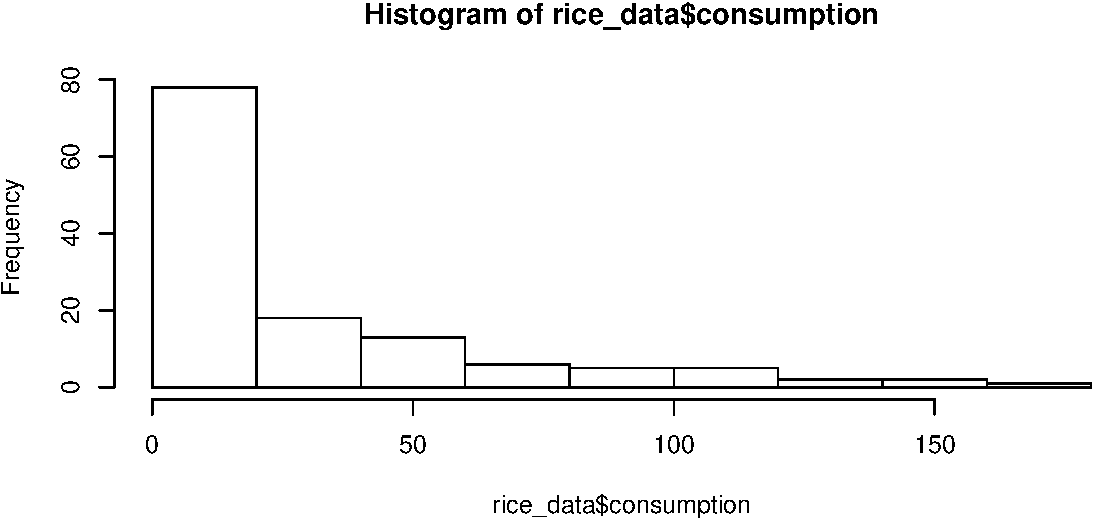
\includegraphics{lecture-03_files/figure-beamer/unnamed-chunk-5-1.pdf}

\end{frame}

\begin{frame}[fragile]{}
\protect\hypertarget{section-12}{}

\textbf{\large Histogram}

Which range of values is most common in our dataset?

\vspace{1ex}\scriptsize

\begin{Shaded}
\begin{Highlighting}[]
\KeywordTok{hist}\NormalTok{(rice_data}\OperatorTok{$}\NormalTok{consumption, }
     \DataTypeTok{xlab =} \StringTok{"Consumption (kg/person/year)"}\NormalTok{,}
     \DataTypeTok{main =} \StringTok{"Histogram of Rice Consumption"}\NormalTok{)}
\end{Highlighting}
\end{Shaded}

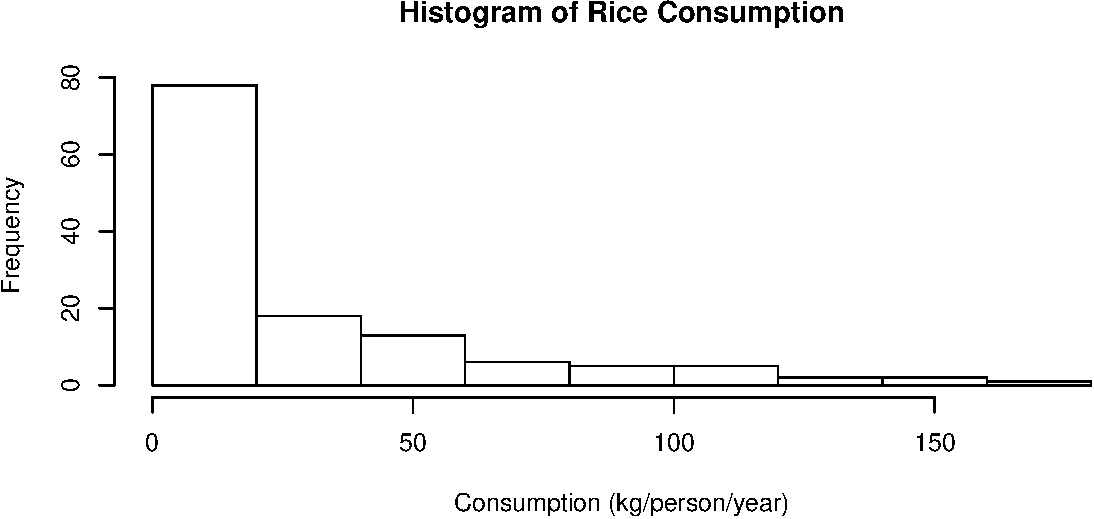
\includegraphics{lecture-03_files/figure-beamer/unnamed-chunk-6-1.pdf}

\end{frame}

\begin{frame}{}
\protect\hypertarget{section-13}{}

\textbf{\large Histogram}

Can we use this plot to make any generalizations about rice consumption
habits in the world?\pause

\vspace{2ex}

\color{coralred} Only if we make statements that are connected to the
types of countries that are well represented in the dataset.

\end{frame}

\begin{frame}{}
\protect\hypertarget{section-14}{}

\textbf{\large Shapes of Histograms}

\vspace{1ex}\scriptsize

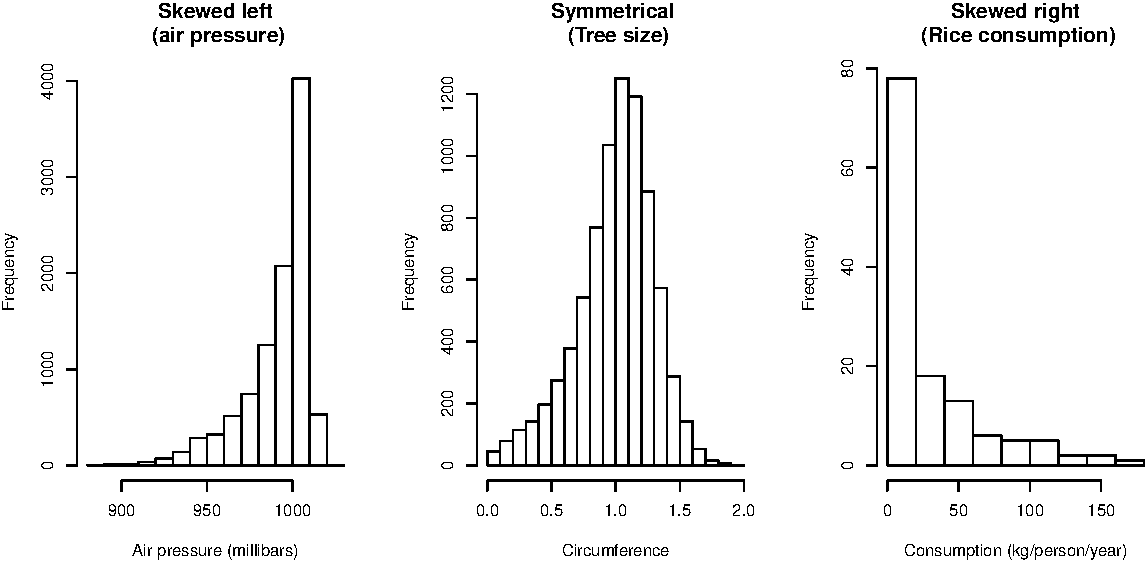
\includegraphics{lecture-03_files/figure-beamer/unnamed-chunk-7-1.pdf}

\end{frame}

\begin{frame}{}
\protect\hypertarget{section-15}{}

\textbf{\large Other Shapes of Histograms}

\vspace{1ex}\scriptsize

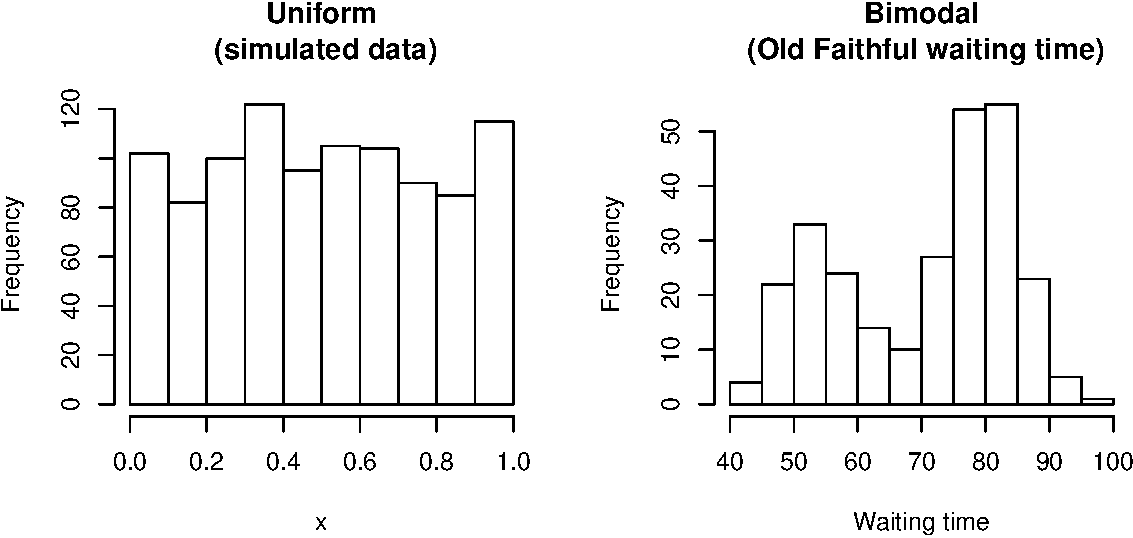
\includegraphics{lecture-03_files/figure-beamer/unnamed-chunk-8-1.pdf}

\end{frame}

\begin{frame}{}
\protect\hypertarget{section-16}{}

\textbf{\large Scatter plot}

Scatter plots illustrate the \textbf{joint distribution} of \textbf{two}
variables at a time, showing which values are relatively more common in
our dataset.

\end{frame}

\begin{frame}[fragile]{}
\protect\hypertarget{section-17}{}

\vspace{1ex}\scriptsize

\begin{Shaded}
\begin{Highlighting}[]
\NormalTok{wheat_data <-}\StringTok{ }\NormalTok{food_consumption }\OperatorTok
\StringTok{  }\KeywordTok{filter}\NormalTok{(food_category }\OperatorTok{==}\StringTok{ "Wheat and Wheat Products"}\NormalTok{)}
\NormalTok{wheat_data}
\end{Highlighting}
\end{Shaded}

\begin{verbatim}
## # A tibble: 130 x 4
##    country     food_category            consumption co2_emmission
##    <chr>       <chr>                          <dbl>         <dbl>
##  1 Argentina   Wheat and Wheat Products       103.           19.7
##  2 Australia   Wheat and Wheat Products        70.5          13.4
##  3 Albania     Wheat and Wheat Products       139.           26.4
##  4 Iceland     Wheat and Wheat Products        72.9          13.9
##  5 New Zealand Wheat and Wheat Products        76.9          14.7
##  6 USA         Wheat and Wheat Products        80.4          15.3
##  7 Uruguay     Wheat and Wheat Products       109.           20.8
##  8 Luxembourg  Wheat and Wheat Products       103.           19.7
##  9 Brazil      Wheat and Wheat Products        53            10.1
## 10 Kazakhstan  Wheat and Wheat Products        92.3          17.6
## # ... with 120 more rows
\end{verbatim}

\end{frame}

\begin{frame}[fragile]{}
\protect\hypertarget{section-18}{}

\textbf{\large Joining data tables}

In order to produce a scatter plot, we need to match countries' wheat
and rice consumption.

\vspace{1ex}\scriptsize

\begin{Shaded}
\begin{Highlighting}[]
\NormalTok{grains_data <-}\StringTok{ }\NormalTok{wheat_data }\OperatorTok
\StringTok{  }\KeywordTok{bind_rows}\NormalTok{(rice_data)}
\NormalTok{grains_data}
\end{Highlighting}
\end{Shaded}

\begin{verbatim}
## # A tibble: 260 x 4
##    country     food_category            consumption co2_emmission
##    <chr>       <chr>                          <dbl>         <dbl>
##  1 Argentina   Wheat and Wheat Products       103.           19.7
##  2 Australia   Wheat and Wheat Products        70.5          13.4
##  3 Albania     Wheat and Wheat Products       139.           26.4
##  4 Iceland     Wheat and Wheat Products        72.9          13.9
##  5 New Zealand Wheat and Wheat Products        76.9          14.7
##  6 USA         Wheat and Wheat Products        80.4          15.3
##  7 Uruguay     Wheat and Wheat Products       109.           20.8
##  8 Luxembourg  Wheat and Wheat Products       103.           19.7
##  9 Brazil      Wheat and Wheat Products        53            10.1
## 10 Kazakhstan  Wheat and Wheat Products        92.3          17.6
## # ... with 250 more rows
\end{verbatim}

\end{frame}

\begin{frame}[fragile]{}
\protect\hypertarget{section-19}{}

\textbf{\large Joining data tables}

What we really want is each row to represent a country, and each column
to represent a type of food. The \texttt{pivot\_wider} function comes in
handy here:

\vspace{1ex}\scriptsize

\begin{Shaded}
\begin{Highlighting}[]
\NormalTok{grains_data <-}\StringTok{ }\NormalTok{grains_data }\OperatorTok
\StringTok{  }\KeywordTok{select}\NormalTok{(}\OperatorTok{-}\NormalTok{co2_emmission) }\OperatorTok\StringTok{ }\CommentTok{# remove c02 variable}
\StringTok{  }\KeywordTok{pivot_wider}\NormalTok{(}\DataTypeTok{names_from =}\NormalTok{ food_category, }\DataTypeTok{values_from =}\NormalTok{ consumption) }\OperatorTok
\StringTok{  }\KeywordTok{rename}\NormalTok{(}\DataTypeTok{Wheat =} \StringTok{`}\DataTypeTok{Wheat and Wheat Products}\StringTok{`}\NormalTok{) }\CommentTok{# make column name shorter}
\end{Highlighting}
\end{Shaded}

\end{frame}

\begin{frame}[fragile]{}
\protect\hypertarget{section-20}{}

\textbf{\large Joining data tables}

What we really want is each row to represent a country, and each column
to represent a type of food.

\vspace{1ex}\scriptsize

\begin{Shaded}
\begin{Highlighting}[]
\KeywordTok{head}\NormalTok{(grains_data)}
\end{Highlighting}
\end{Shaded}

\begin{verbatim}
## # A tibble: 6 x 3
##   country     Wheat  Rice
##   <chr>       <dbl> <dbl>
## 1 Argentina   103.   8.77
## 2 Australia    70.5 11.0 
## 3 Albania     139.   7.78
## 4 Iceland      72.9  3.89
## 5 New Zealand  76.9  9.16
## 6 USA          80.4  6.88
\end{verbatim}

\end{frame}

\begin{frame}[fragile]{}
\protect\hypertarget{section-21}{}

\textbf{\large Scatter plot}

Finally, we can make our scatter plot. What do we observe?

\vspace{1ex}\scriptsize

\begin{Shaded}
\begin{Highlighting}[]
\KeywordTok{plot}\NormalTok{(grains_data}\OperatorTok{$}\NormalTok{Wheat, grains_data}\OperatorTok{$}\NormalTok{Rice,}
     \DataTypeTok{xlab =} \StringTok{"Wheat consumption (kg/person/year)"}\NormalTok{,}
     \DataTypeTok{ylab =} \StringTok{"Rice consumption (kg/person/year)"}\NormalTok{,}
     \DataTypeTok{main =} \StringTok{"Grain consumption"}\NormalTok{,}
     \DataTypeTok{pch =} \DecValTok{16}\NormalTok{, }\DataTypeTok{col =} \StringTok{'tomato'}\NormalTok{)}
\end{Highlighting}
\end{Shaded}

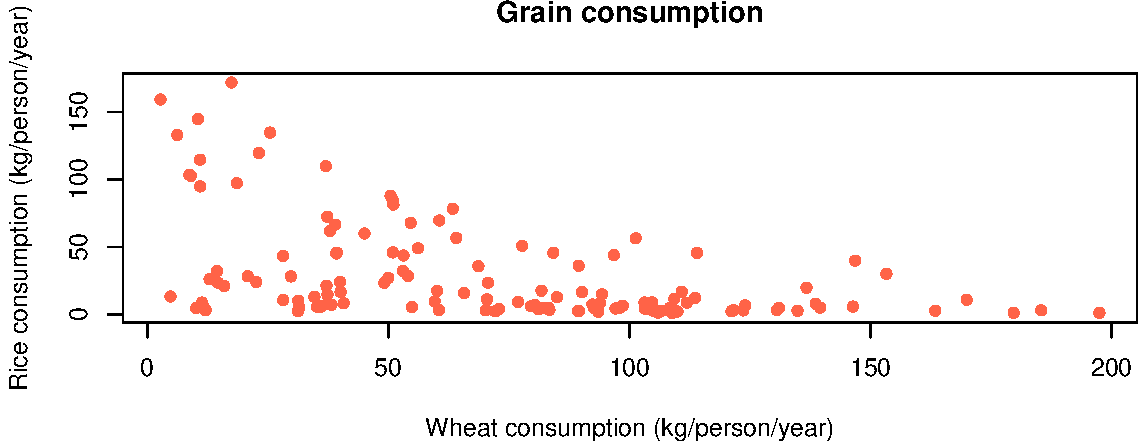
\includegraphics{lecture-03_files/figure-beamer/unnamed-chunk-13-1.pdf}

\end{frame}

\begin{frame}{}
\protect\hypertarget{section-22}{}

\textbf{\large Scatter plot}

For countries in our dataset, there is a \textbf{negative association}
betweeen rice consumption and wheat consumption. Countries that consume
relatively more rice tend consume relatively less wheat.

\vspace{1ex}\scriptsize

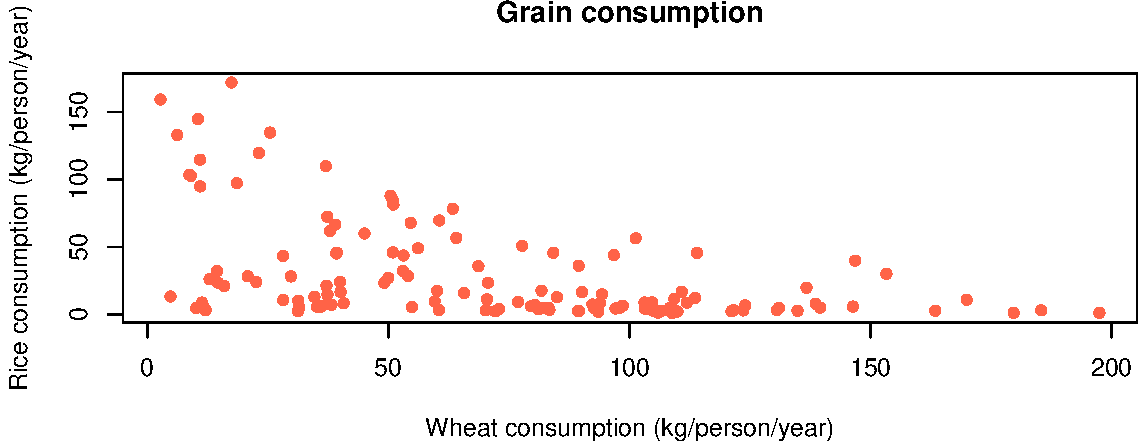
\includegraphics{lecture-03_files/figure-beamer/unnamed-chunk-14-1.pdf}

\end{frame}

\begin{frame}[fragile]{}
\protect\hypertarget{section-23}{}

\textbf{\large Revisiting the histogram}

\vspace{1ex}\scriptsize

\begin{Shaded}
\begin{Highlighting}[]
\KeywordTok{hist}\NormalTok{(grains_data}\OperatorTok{$}\NormalTok{Wheat }\OperatorTok{+}\StringTok{ }\NormalTok{grains_data}\OperatorTok{$}\NormalTok{Rice,}
     \DataTypeTok{xlab =} \StringTok{"Consumption (kg/person/year)"}\NormalTok{,}
     \DataTypeTok{main =} \StringTok{"Wheat and Rice consumption"}\NormalTok{)}
\end{Highlighting}
\end{Shaded}

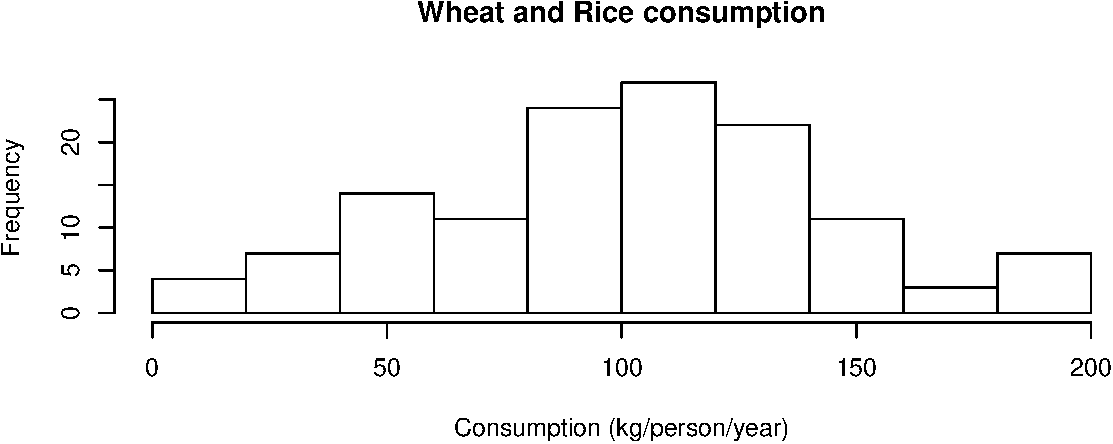
\includegraphics{lecture-03_files/figure-beamer/unnamed-chunk-15-1.pdf}

\end{frame}

\begin{frame}[fragile]{}
\protect\hypertarget{section-24}{}

\textbf{\large Scatter plot in ggplot2}

In case you wanted code to do this in ggplot2.

\vspace{1ex}\scriptsize

\begin{Shaded}
\begin{Highlighting}[]
\KeywordTok{ggplot}\NormalTok{(grains_data) }\OperatorTok{+}
\StringTok{  }\KeywordTok{geom_point}\NormalTok{(}\KeywordTok{aes}\NormalTok{(}\DataTypeTok{x =}\NormalTok{ Wheat, }\DataTypeTok{y =}\NormalTok{ Rice), }\DataTypeTok{color =} \StringTok{'tomato'}\NormalTok{) }\OperatorTok{+}
\StringTok{  }\KeywordTok{xlab}\NormalTok{(}\StringTok{"Wheat consumption (kg/person/year)"}\NormalTok{) }\OperatorTok{+}\StringTok{ }
\StringTok{  }\KeywordTok{ylab}\NormalTok{(}\StringTok{"Rice consumption (kg/person/year)"}\NormalTok{) }\OperatorTok{+}
\StringTok{  }\KeywordTok{ggtitle}\NormalTok{(}\StringTok{"Grain consumption"}\NormalTok{)}
\end{Highlighting}
\end{Shaded}

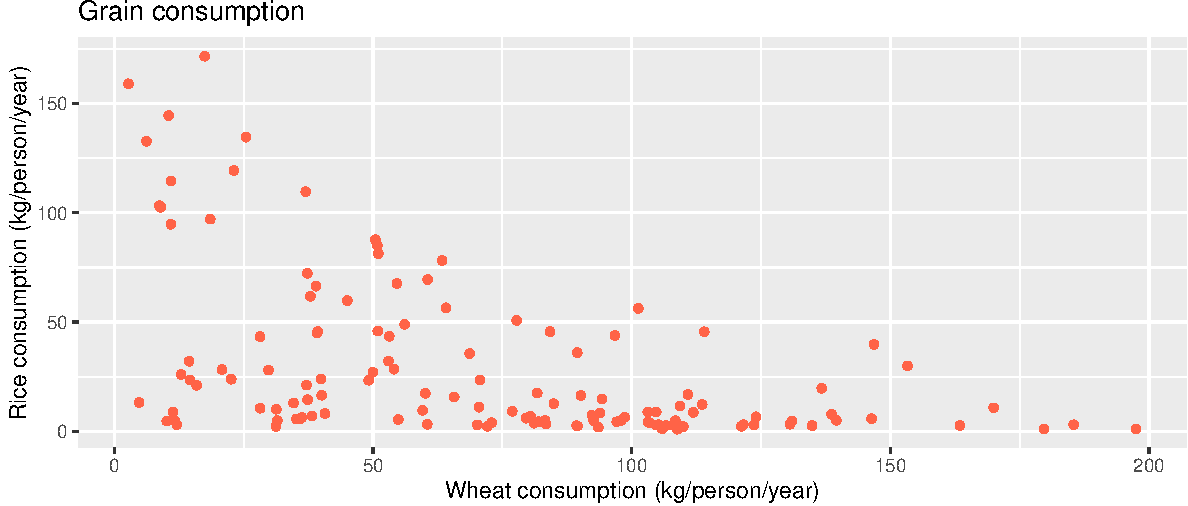
\includegraphics{lecture-03_files/figure-beamer/unnamed-chunk-16-1.pdf}

\end{frame}

\begin{frame}[standout]{}
\protect\hypertarget{section-25}{}

\begin{center}
        
    \vspace{2.3em}
    \color{white}\textit{\Huge\gar Summary statistics}
\end{center}

\end{frame}

\begin{frame}{}
\protect\hypertarget{section-26}{}

\textbf{\large Summary statistics}

\vspace{2ex}

Sometimes we don't want the full \textbf{distribution}: we may just want
a few numbers that summarize our data.

\vspace{2ex}

The full distribution will give us more information, but \textbf{summary
statistics} take up less space and can speed up decision making.

\vspace{2ex}

\textbf{ex.} GPA\pause

\vspace{2ex}

Note that these are all computed based on \textbf{samples} and that we
will focus on statistics for single variables for now.

\end{frame}

\begin{frame}[standout]{}
\protect\hypertarget{section-27}{}

\begin{center}
        
    \vspace{2.3em}
    \color{white}\textit{\Huge\gar ``Location"}
\end{center}

\end{frame}

\begin{frame}{}
\protect\hypertarget{section-28}{}

\textbf{\large Location statistics}

\vspace{2ex}

Some statistics describe the \textbf{location} of our data.

\vspace{2ex}

Crudely speaking, these statistics tell us what possible values of our
variable are the most representative/common/important.

\end{frame}

\begin{frame}{}
\protect\hypertarget{section-29}{}

\textbf{\large Notation}

\vspace{2ex}

Let \(x_1,\ldots, x_n\) denote the \(n\) observations of our variable of
interest.

\end{frame}

\begin{frame}[fragile]{}
\protect\hypertarget{section-30}{}

\textbf{\large Sample mean $\overline{x}$}

\vspace{2ex}

\textbf{In words:} the sum of a collection of numbers divided by the
count of numbers

\vspace{2ex}

\textbf{In math:} \[\overline{x}=\frac{1}{n}\sum_{i=1}^n x_i\]

\vspace{2ex}

\textbf{In R:}

\vspace{1ex}\scriptsize

\begin{Shaded}
\begin{Highlighting}[]
\KeywordTok{mean}\NormalTok{(grains_data}\OperatorTok{$}\NormalTok{Rice)}
\end{Highlighting}
\end{Shaded}

\begin{verbatim}
## [1] 29.37515
\end{verbatim}

\end{frame}

\begin{frame}[fragile]{}
\protect\hypertarget{section-31}{}

\textbf{\large Sample median $\widetilde{x}$}

\vspace{2ex}

\textbf{In words:} the ``middle'' value of a set of numbers

\vspace{2ex}

\textbf{In math:} \begin{align*}
\text{even number of numbers}&: \textrm{median}(\{1, 2, 3,\mathbf{\color{coralred}3}, \mathbf{\color{coralred}5}, 8,8,9\})= \frac{3+5}{2}=4\\
\text{odd number of numbers}&: \textrm{median}(\{3, 4, 4,\mathbf{\color{coralred}5}, 6, 8,9\})= 5\end{align*}

\vspace{2ex}

\textbf{In R:}

\vspace{1ex}\scriptsize

\begin{Shaded}
\begin{Highlighting}[]
\KeywordTok{median}\NormalTok{(grains_data}\OperatorTok{$}\NormalTok{Rice)}
\end{Highlighting}
\end{Shaded}

\begin{verbatim}
## [1] 11.875
\end{verbatim}

\end{frame}

\begin{frame}{}
\protect\hypertarget{section-32}{}

\textbf{\large Sample mode}

\vspace{2ex}

\textbf{In words:} the most common value of a variable

\vspace{2ex}

\textbf{In math:}
\[\textrm{mode}(\{1, 2, \mathbf{\color{coralred}3},\mathbf{\color{coralred}3}, 5\})= 3\]
\[\textrm{mode}(\{1, 2, \mathbf{\color{coralred}3},\mathbf{\color{coralred}3}, 5, \mathbf{\color{coralred}8}, \mathbf{\color{coralred}8},9\})= 3\text{ and } 8\]

\vspace{2ex}

\textbf{In R:} R has no built in mode function!

\end{frame}

\begin{frame}[fragile]{}
\protect\hypertarget{section-33}{}

\textbf{\large Revisiting the histogram}

\vspace{1ex}\scriptsize

\begin{Shaded}
\begin{Highlighting}[]
\KeywordTok{hist}\NormalTok{(grains_data}\OperatorTok{$}\NormalTok{Rice,}
     \DataTypeTok{xlab =} \StringTok{"Consumption (kg/person/year)"}\NormalTok{,}
     \DataTypeTok{main =} \StringTok{"Rice consumption"}\NormalTok{) }
\KeywordTok{abline}\NormalTok{(}\DataTypeTok{v =} \KeywordTok{mean}\NormalTok{(grains_data}\OperatorTok{$}\NormalTok{Rice), }\DataTypeTok{col =} \StringTok{'tomato'}\NormalTok{)}
\KeywordTok{abline}\NormalTok{(}\DataTypeTok{v =} \KeywordTok{median}\NormalTok{(grains_data}\OperatorTok{$}\NormalTok{Rice), }\DataTypeTok{col =} \StringTok{'dodgerblue'}\NormalTok{)}
\KeywordTok{legend}\NormalTok{(}\StringTok{"topright"}\NormalTok{, }\KeywordTok{c}\NormalTok{(}\StringTok{"mean"}\NormalTok{, }\StringTok{"median"}\NormalTok{), }
       \DataTypeTok{col =} \KeywordTok{c}\NormalTok{(}\StringTok{"tomato"}\NormalTok{, }\StringTok{"dodgerblue"}\NormalTok{), }\DataTypeTok{lty =} \DecValTok{1}\NormalTok{)}
\end{Highlighting}
\end{Shaded}

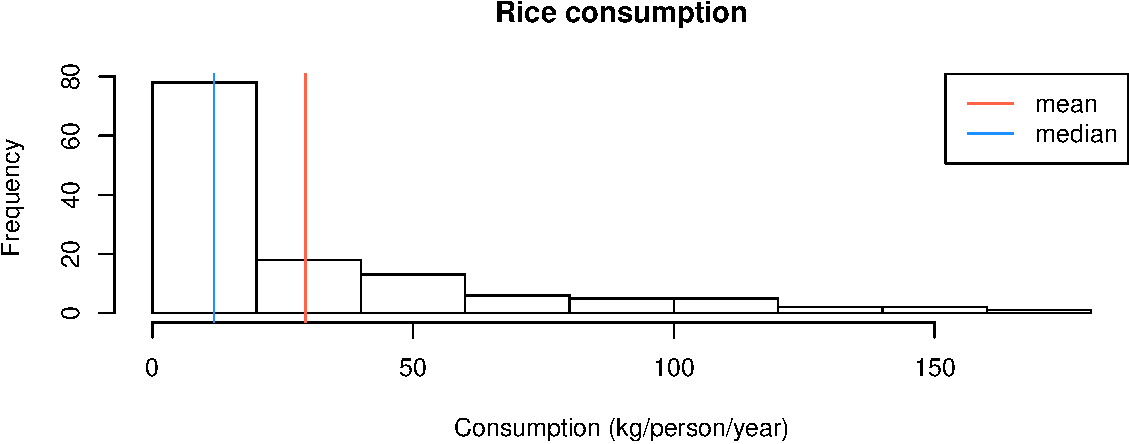
\includegraphics{lecture-03_files/figure-beamer/unnamed-chunk-19-1.pdf}

\end{frame}

\begin{frame}{}
\protect\hypertarget{section-34}{}

\textbf{\large Sensitivity to skew/outliers}

\vspace{2ex}

Imagine that we're all in one classroom (scary!).

\vspace{2ex}

A brave student says:
\textit{I wonder how many Instagram followers the typical person in this room has.}

\vspace{2ex}

Another over-eager student says:
\textit{Let's take a sample of 10 people and find out!}

\vspace{2ex}

What sample location statistic should we calculate based on our sample?

\end{frame}

\begin{frame}{}
\protect\hypertarget{section-35}{}

\textbf{\large Sensitivity to skew/outliers}

\vspace{2ex}

Now, suppose Christiano Ronaldo (225 million), Ariana Grande (191.1 m),
The Rock (187.3 m) walk into the room.

\vspace{2ex}

They would be \textbf{outliers} in our population, meaning that their
values would be located abnormally far from the other values.

\vspace{2ex}

Suppose they all end up in our sample. What happens to the sample mean?
What happens to the sample median?

\end{frame}

\begin{frame}[fragile]{}
\protect\hypertarget{section-36}{}

\textbf{\large Comparing location statistics}

\vspace{1ex}\scriptsize

\begin{Shaded}
\begin{Highlighting}[]
\KeywordTok{hist}\NormalTok{(grains_data}\OperatorTok{$}\NormalTok{Rice,}
     \DataTypeTok{xlab =} \StringTok{"Consumption (kg/person/year)"}\NormalTok{,}
     \DataTypeTok{main =} \StringTok{"Rice consumption"}\NormalTok{) }
\KeywordTok{abline}\NormalTok{(}\DataTypeTok{v =} \KeywordTok{mean}\NormalTok{(grains_data}\OperatorTok{$}\NormalTok{Rice), }\DataTypeTok{col =} \StringTok{'tomato'}\NormalTok{)}
\KeywordTok{abline}\NormalTok{(}\DataTypeTok{v =} \KeywordTok{median}\NormalTok{(grains_data}\OperatorTok{$}\NormalTok{Rice), }\DataTypeTok{col =} \StringTok{'dodgerblue'}\NormalTok{)}
\KeywordTok{legend}\NormalTok{(}\StringTok{"topright"}\NormalTok{, }\KeywordTok{c}\NormalTok{(}\StringTok{"mean"}\NormalTok{, }\StringTok{"median"}\NormalTok{), }
       \DataTypeTok{col =} \KeywordTok{c}\NormalTok{(}\StringTok{"tomato"}\NormalTok{, }\StringTok{"dodgerblue"}\NormalTok{), }\DataTypeTok{lty =} \DecValTok{1}\NormalTok{)}
\end{Highlighting}
\end{Shaded}

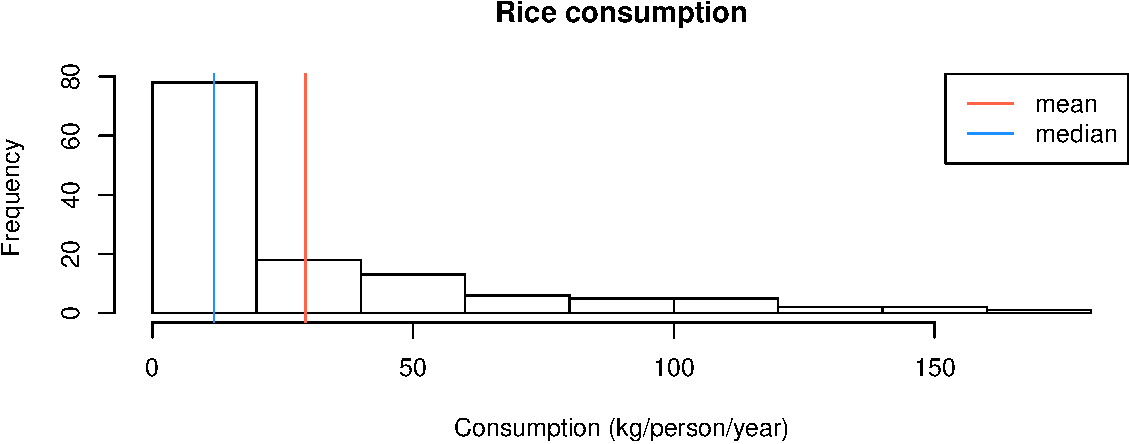
\includegraphics{lecture-03_files/figure-beamer/unnamed-chunk-20-1.pdf}

\end{frame}

\begin{frame}{}
\protect\hypertarget{section-37}{}

\textbf{\large Comparing location statistics}

\vspace{2ex}
\scriptsize
\begin{tabular}{|r|p{.27\textwidth}|p{.27\textwidth}|p{.24\textwidth}|}
\hline
Statistic & Mean & Median & Mode\\
\hline
Pros & 
\begin{itemize}[leftmargin=*]\item[]  - unique value
\item[] - good for inference\end{itemize} & 
\begin{itemize}[leftmargin=*]\item[] - unique value
\item[] - robust to outliers \end{itemize} & 
\begin{itemize}[leftmargin=*]\item[]  - easy to explain 
\item[] - can compute for numerical and categorical variables\end{itemize}\\\hline
Cons & 
\begin{itemize}[leftmargin=*]\item[]  - sensitive to outliers \item - only numerical variables
\end{itemize} & 
\begin{itemize}[leftmargin=*]\item - only numerical variables\end{itemize} & 
\begin{itemize}[leftmargin=*]\item[]  - may not be unique/meaningful\end{itemize}\\\hline
\end{tabular}

\end{frame}

\begin{frame}{}
\protect\hypertarget{section-38}{}

\textbf{\large Other location statistics}

\textbf{Quartiles} split your data up into quarters. If you think of the
median as the second quartile, then the first quartile is the median of
the first half of the data and third quartile is the median of the
second half of the data.

\vspace{2ex}

So, 25\% of the data fall below the first quartile and 75\% fall below
the third quartile.

\end{frame}

\begin{frame}{}
\protect\hypertarget{section-39}{}

\textbf{\large Boxplots}

We can use boxplots to summarize distributions and visualize the
quartiles:

\vspace{1ex}

The edges of the box represent the first and third quartile

\vspace{1ex}

The line inside the box is the median

\vspace{1ex}

The edges of the ``whiskers'' are usually the maximum and minimum

\vspace{1ex}\scriptsize

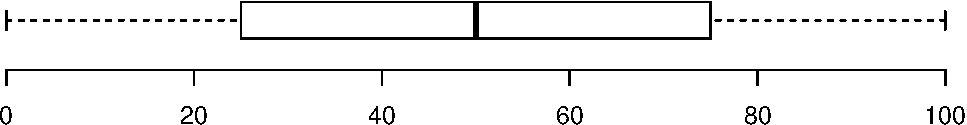
\includegraphics{lecture-03_files/figure-beamer/unnamed-chunk-21-1.pdf}

\end{frame}

\begin{frame}{}
\protect\hypertarget{section-40}{}

\textbf{\large Boxplots}

Returning to our rice consumption data (the points to the right are
\textbf{outliers}):

\vspace{1ex}\scriptsize

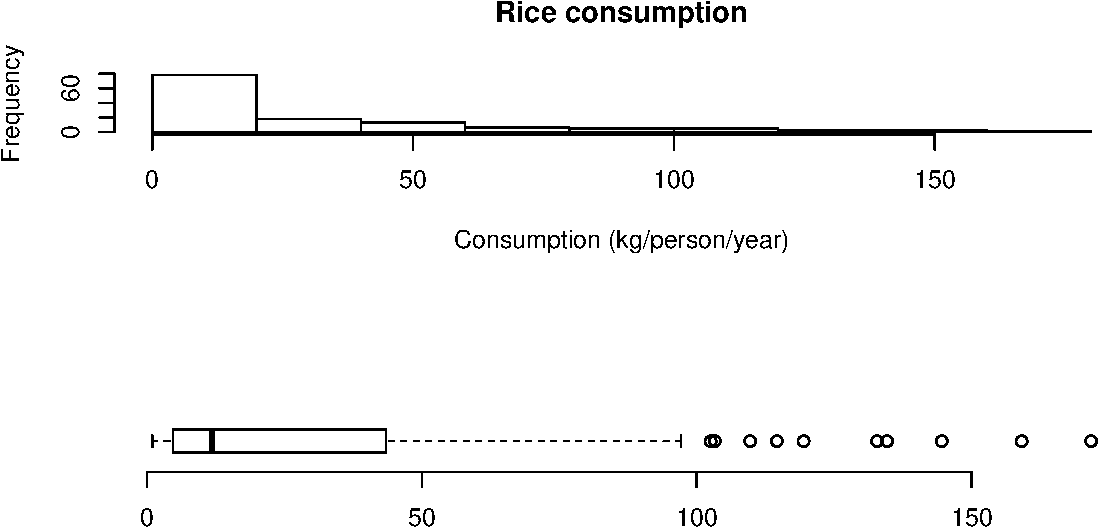
\includegraphics{lecture-03_files/figure-beamer/unnamed-chunk-22-1.pdf}

\end{frame}

\begin{frame}{}
\protect\hypertarget{section-41}{}

\textbf{\large Example Boxplots}

\vspace{1ex}\scriptsize

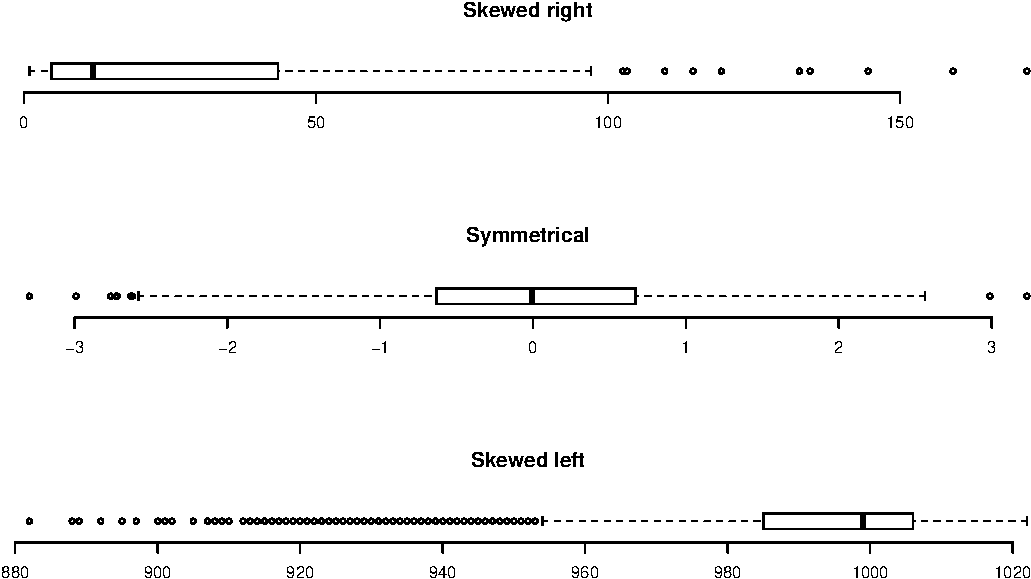
\includegraphics{lecture-03_files/figure-beamer/unnamed-chunk-23-1.pdf}

\end{frame}

\begin{frame}[standout]{}
\protect\hypertarget{section-42}{}

\begin{center}
    \vspace{2.3em}
    \color{white}\textit{\Huge\gar ``Spread"}
\end{center}

\end{frame}

\begin{frame}{}
\protect\hypertarget{section-43}{}

\textbf{\large Spread statistics}

\vspace{2ex}

Some statistics describe the \textbf{location} of our data.

\vspace{2ex}

Crudely speaking, these statistics tell us how far our data values tend
to be from each other.

\end{frame}

\begin{frame}[fragile]{}
\protect\hypertarget{section-44}{}

\textbf{\large Range}

\vspace{2ex}

\textbf{In words:} the difference between the biggest data value and the
smallest data value

\vspace{2ex}

\textbf{In math:}
\[\textrm{range}(x_1,\ldots, x_n)=\max(x_1,\ldots, x_n) - \min(x_1,\ldots, x_n)\]

\vspace{2ex}

\textbf{In R:}

\vspace{1ex}\scriptsize

\begin{Shaded}
\begin{Highlighting}[]
\KeywordTok{range}\NormalTok{(grains_data}\OperatorTok{$}\NormalTok{Rice)}
\end{Highlighting}
\end{Shaded}

\begin{verbatim}
## [1]   0.95 171.73
\end{verbatim}

\end{frame}

\begin{frame}{}
\protect\hypertarget{section-45}{}

\textbf{\large Sample Variance}

\vspace{2ex}

Let the \textbf{sample deviation} be the distance of an observation from
its sample mean. So, for now, we compute the sample deviation of \(x_i\)
as \(x_i-\overline{x}\).

\vspace{2ex}

We define \textbf{sample variance} as the average squared sample
deviation of the observations.

\end{frame}

\begin{frame}[fragile]{}
\protect\hypertarget{section-46}{}

\textbf{\large Sample Variance}

\vspace{2ex}

\textbf{In words:} the ``average'' squared deviation of the observations

\vspace{2ex}

\textbf{In math:}
\[\textrm{Var}(x_1,\ldots, x_n)=\frac{1}{n-1}\sum_{i=1}^n(x_i-\overline{x})^2\]
\hfill\textbf{\color{coralred} Note: we divide by $n-1$ to get a better estimator}

\vspace{2ex}

\textbf{In R:}

\vspace{1ex}\scriptsize

\begin{Shaded}
\begin{Highlighting}[]
\KeywordTok{var}\NormalTok{(grains_data}\OperatorTok{$}\NormalTok{Rice)}
\end{Highlighting}
\end{Shaded}

\begin{verbatim}
## [1] 1393.116
\end{verbatim}

\end{frame}

\begin{frame}[fragile]{}
\protect\hypertarget{section-47}{}

\textbf{\large Sample Standard Deviation}

\vspace{2ex}

\textbf{In words:} the square root of ``average'' squared deviation of
the observations

\vspace{2ex}

\textbf{In math:}
\[\textrm{SD}(x_1,\ldots, x_n)=\sqrt{\frac{1}{n-1}\sum_{i=1}^n(x_i-\overline{x})^2}\]
\hfill\textbf{\color{coralred} Note: we divide by $n-1$ to get a better estimator}

\vspace{2ex}

\textbf{In R:}

\vspace{1ex}\scriptsize

\begin{Shaded}
\begin{Highlighting}[]
\KeywordTok{sd}\NormalTok{(grains_data}\OperatorTok{$}\NormalTok{Rice)}
\end{Highlighting}
\end{Shaded}

\begin{verbatim}
## [1] 37.32447
\end{verbatim}

\end{frame}

\begin{frame}{}
\protect\hypertarget{section-48}{}

Which data has the higher standard deviation?

\vspace{1ex}\scriptsize

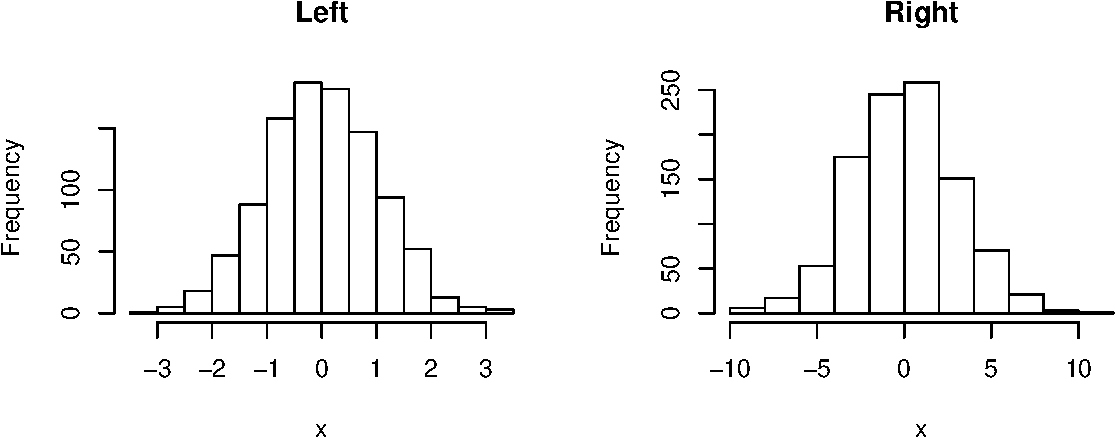
\includegraphics{lecture-03_files/figure-beamer/unnamed-chunk-27-1.pdf}

\end{frame}

\begin{frame}{}
\protect\hypertarget{section-49}{}

Drawn on the same scale:

\vspace{1ex}\scriptsize

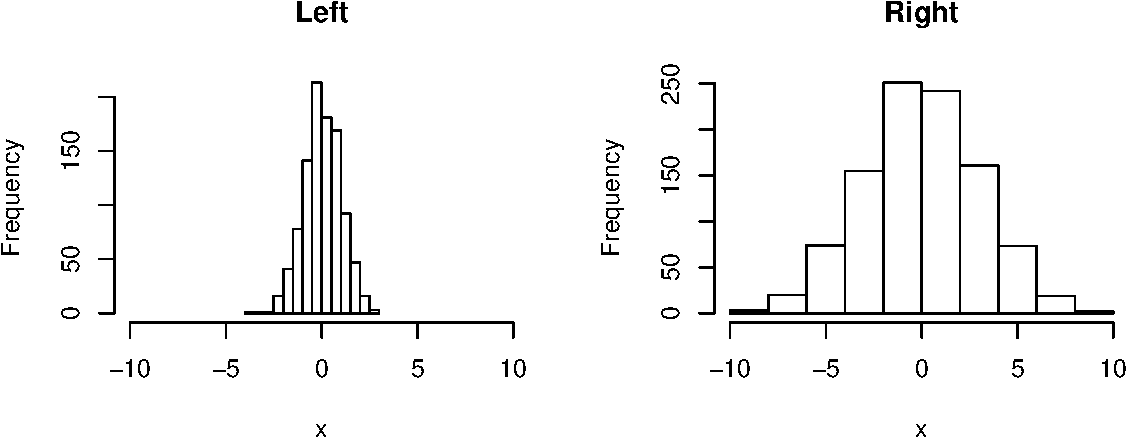
\includegraphics{lecture-03_files/figure-beamer/unnamed-chunk-28-1.pdf}

\end{frame}

\begin{frame}{}
\protect\hypertarget{section-50}{}

\textbf{\large Context matters}

Context matters a lot when discussing standard deviation. These two
(fake) datasets have the same standard deviation:

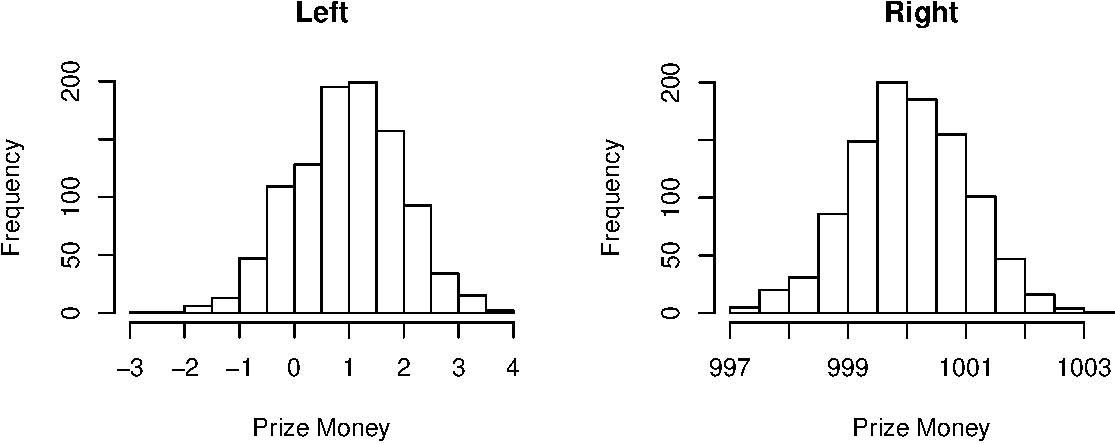
\includegraphics{lecture-03_files/figure-beamer/unnamed-chunk-29-1.pdf}

\end{frame}

\begin{frame}[fragile]{}
\protect\hypertarget{section-51}{}

\textbf{\large Coefficient of variation}

\vspace{2ex}

\textbf{In words:} the standard deviation divided by the mean

\vspace{2ex}

\textbf{In math:}
\[\textrm{CV}(x_1,\ldots, x_n)=\frac{\textrm{SD}(x_1,\ldots, x_n)}{\overline{x}}\]
\vspace{2ex}\textbf{In R:}

\vspace{1ex}\scriptsize

\begin{Shaded}
\begin{Highlighting}[]
\KeywordTok{sd}\NormalTok{(grains_data}\OperatorTok{$}\NormalTok{Rice) }\OperatorTok{/}\StringTok{ }\KeywordTok{mean}\NormalTok{(grains_data}\OperatorTok{$}\NormalTok{Rice)}
\end{Highlighting}
\end{Shaded}

\begin{verbatim}
## [1] 1.270614
\end{verbatim}

\end{frame}

\begin{frame}[standout]{}
\protect\hypertarget{section-52}{}

\color{apricot}\textit{\gar\Huge recap}

\normalsize\color{white}\vspace{4ex}\textbf{Today, we discussed:}

\vspace{2ex}
\begin{itemize}
\color{white}
\setlength{\itemsep}{2ex}
\item Visualizing distributions
\item Location statistics
\item Spread statistics
\end{itemize}

\end{frame}

\begin{frame}[standout]{}
\protect\hypertarget{section-53}{}

\color{apricot}\textit{\gar\Huge recap}

\normalsize\color{white}\vspace{4ex}\textbf{If you only take one thing away from today:}

\vspace{2ex}

All of the summaries/statistics we discussed today were calculated
without making \textbf{any assumptions} about our population. \pause

\vspace{2ex}

All were based entirely on our \textbf{sample}. In the next lecture
we'll talk more about how we can use \textbf{sample statistics} to
estimate \textbf{population parameters}.

\end{frame}

\end{document}
